\chapter{Ejercicio Sigue Personas Real en Robotics Academy}
\label{cap:capitulo6}

En este capítulo nos centraremos en la implementación del ejercicio \textit{Real Follow Person} en Robotics Academy. Al tratarse de un ejercicio semejante al del capítulo 5, explicaremos aquellos cambios relevantes aplicados tanto en el módulo HAL como en la solución de referencia. Además, hablaremos de la incorporación del Turtlebot2 en las imágenes RADI (de Docker) que permite al usuario con solo usar el navegador acceder al hardware real del robot.\\



% -- INTEGRACION DOCKER
% -----------------------
\section{Integración Turtlebot2 en Docker}
\label{sec:integracion_turtlebot2_docker}

Para conseguir la conexión con el robot vía Docker se ha incluido en los ficheros Dockerfile algunos repositorios de terceros:

\begin{itemize}
	\item Para controlar la base \textit{Kobuki} se ha necesitado el repositorio de \textit{kobuki\_ros} que se ha integrado previamente en \textit{Custom Robots}\footnote{\textbf{CustomRobots}: \url{https://github.com/JdeRobot/CustomRobots/tree/foxy-devel}} de JdeRobot.
	
	\item Para usar el láser RPLIDAR A1, se ha usado el repositorio \textit{rplidar\_ros}\footnote{\textbf{Rplidar\_ros}: \url{https://github.com/allenh1/rplidar_ros}} del usuario de Github \textit{allenh1} en su rama para ROS2. Para integrarlo en el fichero Dockerfile se ha usado el comando \textit{sed} de Linux para cambiar el dispositivo por defecto (/dev/ttyUSB0 a /dev/ttyUSB1) en el fichero de lanzamiento rplidar.launch.py.
\begin{code}[H]
\begin{lstlisting}
RUN cd /opt/jderobot/CustomRobots && \
	git clone https://github.com/allenh1/rplidar_ros.git -b ros2 && \
	cd rplidar_ros/launch && \
	sed -i "$(grep -n serial_port rplidar.launch.py | cut -d: -f1) s/\/dev\/ttyUSB0/\/dev\/ttyUSB1/g" rplidar.launch.py
\end{lstlisting}
\caption{Integración del RPLIDAR A1 en el fichero Dockerfile}
\label{cod:rplidar_dockerfile}
\end{code}

	\item Para usar la cámara IntelRealsense R200 solo hemos necesitado incluir en el fichero Dockerfile-foxy.base el comando de instalación del paquete de ROS2 \textit{ros-foxy-v4l2-camera} que sirve para publicar sobre un \textit{topic} (/image\_raw) los fotogramas de la cámara a una frecuencia de 60 Hz.
\end{itemize}\

Una vez instaladas las dependencias y creada una imagen Docker, se ha de tener en cuenta los dispositivos conectados en el portátil del usuario para el lanzamiento del contenedor. Para indicar al contenedor que dispositivos del sistema operativo queremos integrar dentro del sistema virtualizado usaremos el parámetro --device. Cuando usemos el robot real, tendremos que seguir las siguientes reglas en el siguiente orden (preferiblemente):

\begin{itemize}
	\item Base \textit{Kobuki}. Al encender la base \textit{Kobuki} y conectarla al portátil, su conexión abrirá el dispositivo /dev/ttyUSB0.
	\item \textit{RPLIDAR A1}. Al conectar su cable USB después de conectar la base Kobuki se habilitará el dispositivo /dev/ttyUSB1.
	\item Cámara \textit{Intel Realsense R200}. Su conexión abré 6 dispositivos /dev/video[0-5]. Nosotros nos quedaremos con /dev/video4 cuya salida se muestra en el espacio de color RGB (comprobado con este comando \footnote{\textbf{cvlc v4l2:///dev/video4}}). Como se ha integrado en Robotics Academy para las cámara que abran el dispositivo /dev/video0 tendremos que usar un remapeo: /dev/video4:/dev/video0.
\end{itemize}\

El comando para lanzar el ejercio \textit{Real Follow Person} usando la cámara R200 será el siguiente (para otras cámaras el remapeo puede ser distinto):\\

\begin{code}[H]
\begin{lstlisting}
$>  docker run -it --device /dev/ttyUSB0 --device /dev/ttyUSB1 --device /dev/video4:/dev/video0 -p 8000:8000 -p 2303:2303 -p 1905:1905 -p 8765:8765 -p 6080:6080 -p 1108:1108 jderobot/robotics-academy:4.3.0 ./start.sh
\end{lstlisting}
\caption{Lanzamiento del RADI 4 para usar Real Follow Person}
\label{cod:lanzamiento_radi_real_follow_person}
\end{code}

Una vez lanzado el contenedor, podremos acceder a la plantilla web del ejercicio y comenzar a programar sobre el robot real. En la plantilla web tendremos como GUI, un \textit{canvas} para visualizar los fotogramas de la cámara y un terminal (mediante conexión VNC) para depurar.

\begin{figure} [H]
	\begin{center}
		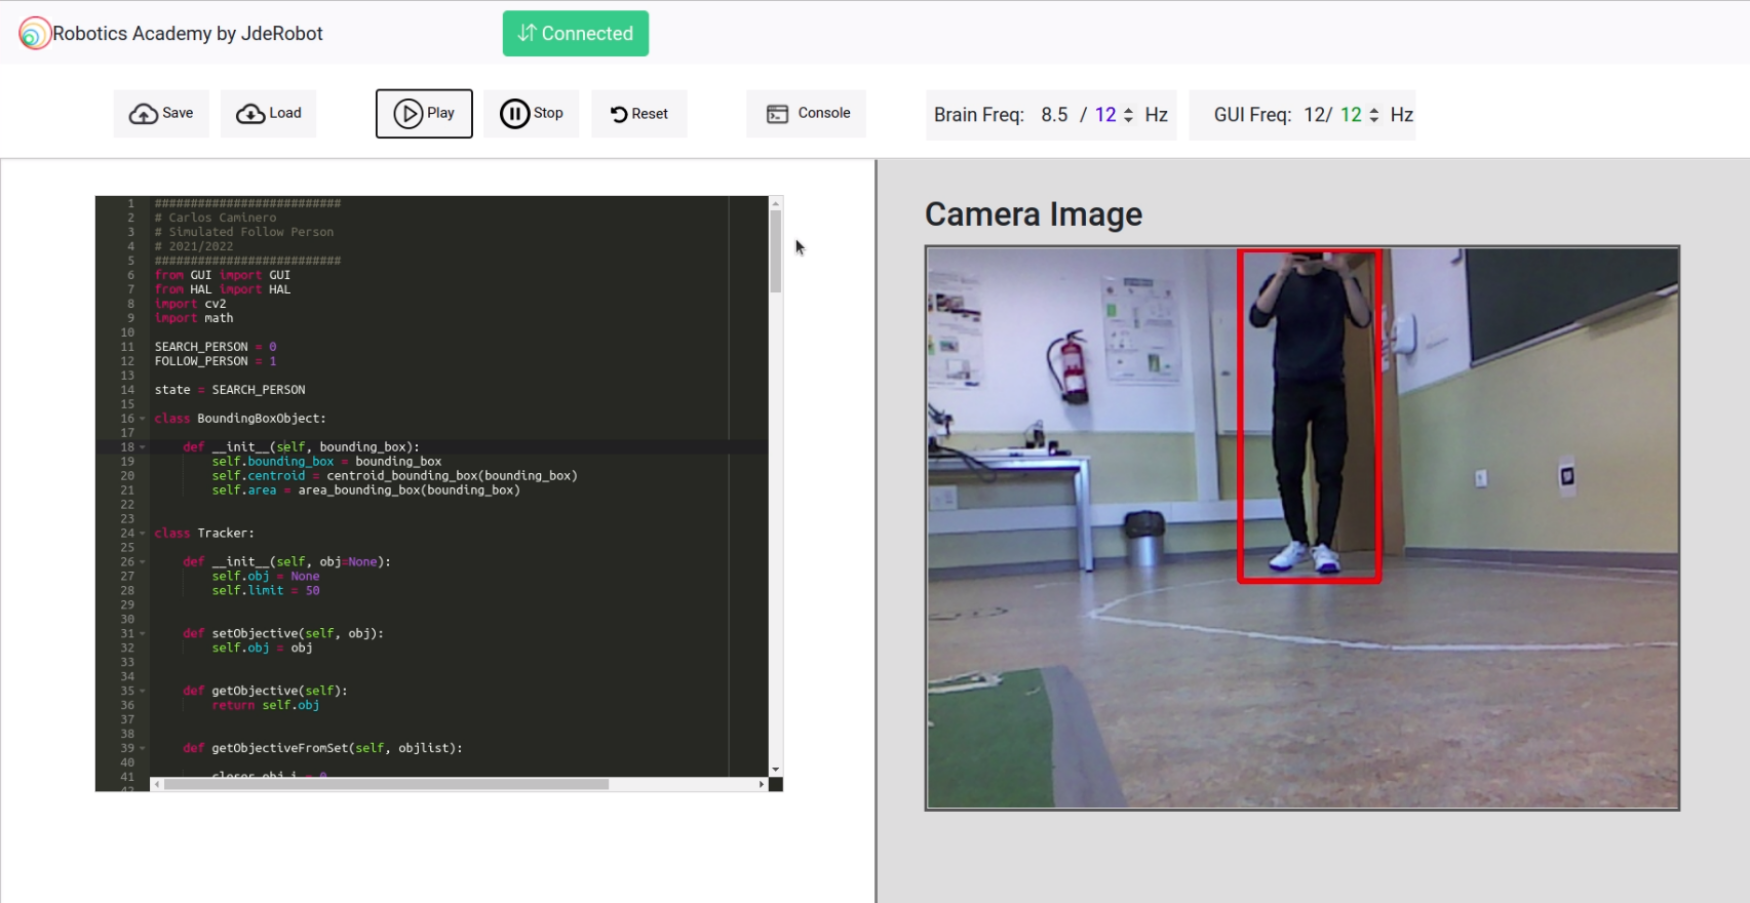
\includegraphics[width=12cm]{imagenes/cap6/plantilla-web.png}
	\end{center}
	\caption[Plantilla web del ejercicio Real Follow Person]{Plantilla web del ejercicio Real Follow Person}
	\label{fig:plantilla_web_real_follow_person}
\end{figure}\




% -- SECCION HAL
% ----------------
\section{HAL y solución de referencia}
\label{sec:hal_solucion_real_follow_person}

La infraestructura del ejercicio es muy parecida al del ejercicio Follow Person simulado, de modo que describiremos los cambios más relevantes:

\begin{itemize}
	\item Ausencia del simulador Gazebo debido al uso de un robot físico y su ejecución sobre un escenario real. Ello implica un incremento de velocidad de procesamiento al no saturar de procesos el sistema virtualizado.
	\item Cambio en los tópics de publicación y suscripción en el módulo HAL:
	\begin{itemize}
		\item La velocidad se publica en el \textit{topic} /commands/velocity. El nodo de la base \textit{Kobuki} (fichero kobuki\_ros.cpp del paquete kobuki\_node) se suscribe al topic y comanda directamente las velocidades al hardware: \textit{kobuki\_.setBaseControl(msg-$>$linear.x, msg-$>$angular.z)};
		\item Las lecturas del láser se obtienen del mismo \textit{topic} /scan.
		\item Los fotogramas de la cámara se obtienen del \textit{topic} /image\_raw que se genera cuando lanzamos el nodo v4l2\_camera\_node sobre el dispositivo /dev/video0
		\item La odometría del robot se obtiene del mismo \textit{topic}: /odom.
	\end{itemize}
	\item Cambio en la configuración del láser en la función HAL.getLaserData(). Durante las pruebas realizadas con el robot real, fue necesario volver a ajustar la dirección de las lecturas del láser tal y como hicimos en el capítulo 5 [\ref{sec:hal_sim_follow_person}] y poder devolver 180 lecturas en un orden correcto:
	\begin{code}[H]
	\begin{lstlisting}
	def getLaserData(self):
		values = self.laser.getLaserData().values
		return values[270:360:1] + values[0:1] + values[1:90:1]
	\end{lstlisting}
	\caption{Módulo HAL en Real Follow Person: getLaserData}
	\label{cod:real_follow_person_hal_laser}
	\end{code}
\end{itemize}

En la \textit{solución} de referencia seguimos los mismos pasos que en la sección [\ref{sec:sigue_personas_simulado}]:
\begin{itemize}
	\item Implementación del \textit{Tracker} de seguimiento. Los pasos son los mismos:
	\begin{enumerate}
		\item Localizar a una persona aplicando los filtros de \textit{score} o puntuación, cláse y área.
		\item Aplicaremos el criterio de \textit{selección}: dividir la imagen en 3 secciones y elegir como objetivo la persona más cercana que esté situada en la sección central
		\item Crear una clase Tracker que guarde constantemente y vaya actualizando el objetivo de seguimiento por cada fotograma.
		\item Para no perder al objetivo, en cada fotograma nos quedaremos con el centroide del \textit{Bounding Box} más cercano al centroide candidato del fotograma anterior, mientras no supere un límite de distancia. En caso de no detectar al objetivo, iremos incrementando un contador de fallo.
	\end{enumerate}
	\begin{figure} [H]
		\begin{center}
			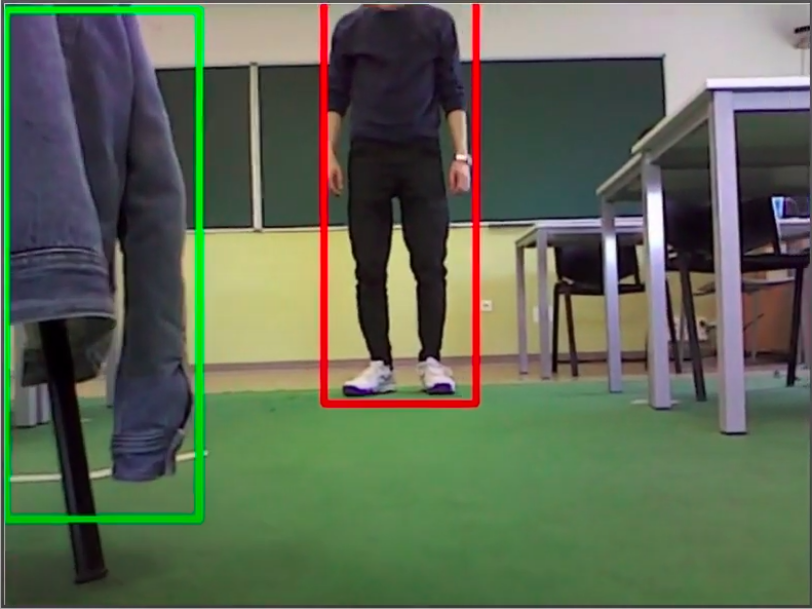
\includegraphics[width=10cm]{imagenes/cap6/tracker.png}
		\end{center}
		\caption[Tracker en el ejercicio Real Follow Person]{Tracker en el ejercicio Real Follow Person}
		\label{fig:tracker_real_follow_person}
	\end{figure}\
	
	\item Implementación del algoritmo VFF. Como la frecuencia de actualización cambia ante la ausencia del simulador, ha sido necesario reajustar los parámetros $\alpha$ y $\beta$ del algoritmo, para equilibrar la relación entre la fuerza de atracción y de repulsión.
	
	\item Máquina de Estados Finitos. Seguimos usando dos estados maestros: Buscar-Persona y Seguir-Persona. La transición del estado Seguir-Persona a Buscar-Persona estaba determinado por el contador de fallo que indiciamos en el proceso de seguimiento del Tracking. El límite del contador dependerá de los fotogramas por segundo. En el ejercicio \textit{Follow Person} simulado, la velocidad de fotogramas era baja por lo tanto el límite era menor, pero en este caso, al haber aumentado la velocidad de refresco, tiene sentido aumentar el límite del contador para que, de esta manera, si perdemos a la persona en un fotograma, podamos seguir guardando el centroide del útlimo \textit{Bounding Box} candidato.
\end{itemize}\

El resultado de la solución podemos verlo en el siguiente enlace:\\
\textit{\url{https://youtu.be/54Jb4KJwyDM}}\\

Con este nuevo ejercicio y el anterior se pretende poner en práctica la experiencia del programador de robots cuando desarrolla una solución robótica. El primer paso es probar su programa en una simulación (ejemplo de Follow Person simulado), una vez que su solución es bastante robusta, pasa al siguiente nivel, probandolo en el mundo real (Real Follow Person). El programador se dará cuenta de que es muy probable que el mismo programa en simulación no funcione igual que con un robot real. Entonces, si su solución era bastante buena, solamente tendrá que ajustar algunos parámetros y tener en cuenta ciertos factores (como el terreno) y habrá logrado su objetivo.\\